%%%%%%%%%%%%%%%%%%%%%%%%%%%%%%%%%%%%%%%%%%%%%%%%%%%%%%%%%%%%%%%%%%%%%%%%%%%%%%%
\section{Generality with respect to the spatial discretization}
\label{sec:spatial-generality}
%%%%%%%%%%%%%%%%%%%%%%%%%%%%%%%%%%%%%%%%%%%%%%%%%%%%%%%%%%%%%%%%%%%%%%%%%%%%%%%

The preceding mechanism was derived first for the cubic-B-spline de Frutos
operator.  We now test whether it is tied to that particular stencil.  We use
the four compact discretizations compared in the earlier study of numerical
compacton radiation: Ismail--Taha, de Frutos, Pad\'e-6, and Pad\'e-8, with
formal derivative orders $(2,2)$, $(6,4)$, $(4,6)$, and $(8,2)$,
respectively.  The nonlinear flux and the implicit or Gauss time integrator
are otherwise unchanged.

\subsection{Method-dependent Nyquist solitary families}

Exact demodulation $U_j=(-1)^j a_j$ applies to all four centered stencils.  A
traveling envelope satisfies
\begin{equation}
 V_{i,h}F_i=\mathcal M_{i,h}(F_i^2),
 \qquad
 v=\frac{A}{h^2}V_{i,h},
 \label{eq:wp4-family}
\end{equation}
where
\begin{align}
\mathcal M_{\rm IT,h}(D)
 &=\frac{\sinh D}{D}\,[2(\cosh D+1)-h^2],\\
\mathcal M_{\rm DF,h}(D)
 &=10\frac{\sinh D}{D}
 \frac{(h^2+12)\cosh D-5h^2+12}
      {\cosh(2D)-26\cosh D+33},\\
\mathcal M_{\rm P6,h}(D)
 &=20\frac{\sinh D}{D}
 \frac{(h^2+12)\cosh D-5h^2+12}
      {\cosh(2D)-56\cosh D+63},\\
\mathcal M_{\rm P8,h}(D)
 &=\frac53\frac{\sinh D}{D}
 \frac{42(\cosh D+1)+h^2(5\cosh D-16)}
      {\cosh(2D)-16\cosh D+18}.
 \label{eq:wp4-operators}
\end{align}
Figure~\ref{fig:wp4-profiles} shows that the normalized profiles are visibly
stencil dependent.  At $h=0.02$, their velocity coefficients are
\begin{equation}
 V_{\rm IT}=2.8576467,\quad
 V_{\rm DF}=20.6605217,\quad
 V_{\rm P6}=40.7496398,\quad
 V_{\rm P8}=31.9901995,
 \label{eq:wp4-V}
\end{equation}
with FWHM values $3.186$, $5.449$, $7.295$, and $6.196$ grid cells.  The
relative residuals of the four profile equations are below $3.1\times10^{-13}$.
Thus the scaling $v\propto A/h^2$ is structural, but its coefficient and the
wave shape are properties of the spatial discretization.

\begin{figure}[t]
 \centering
 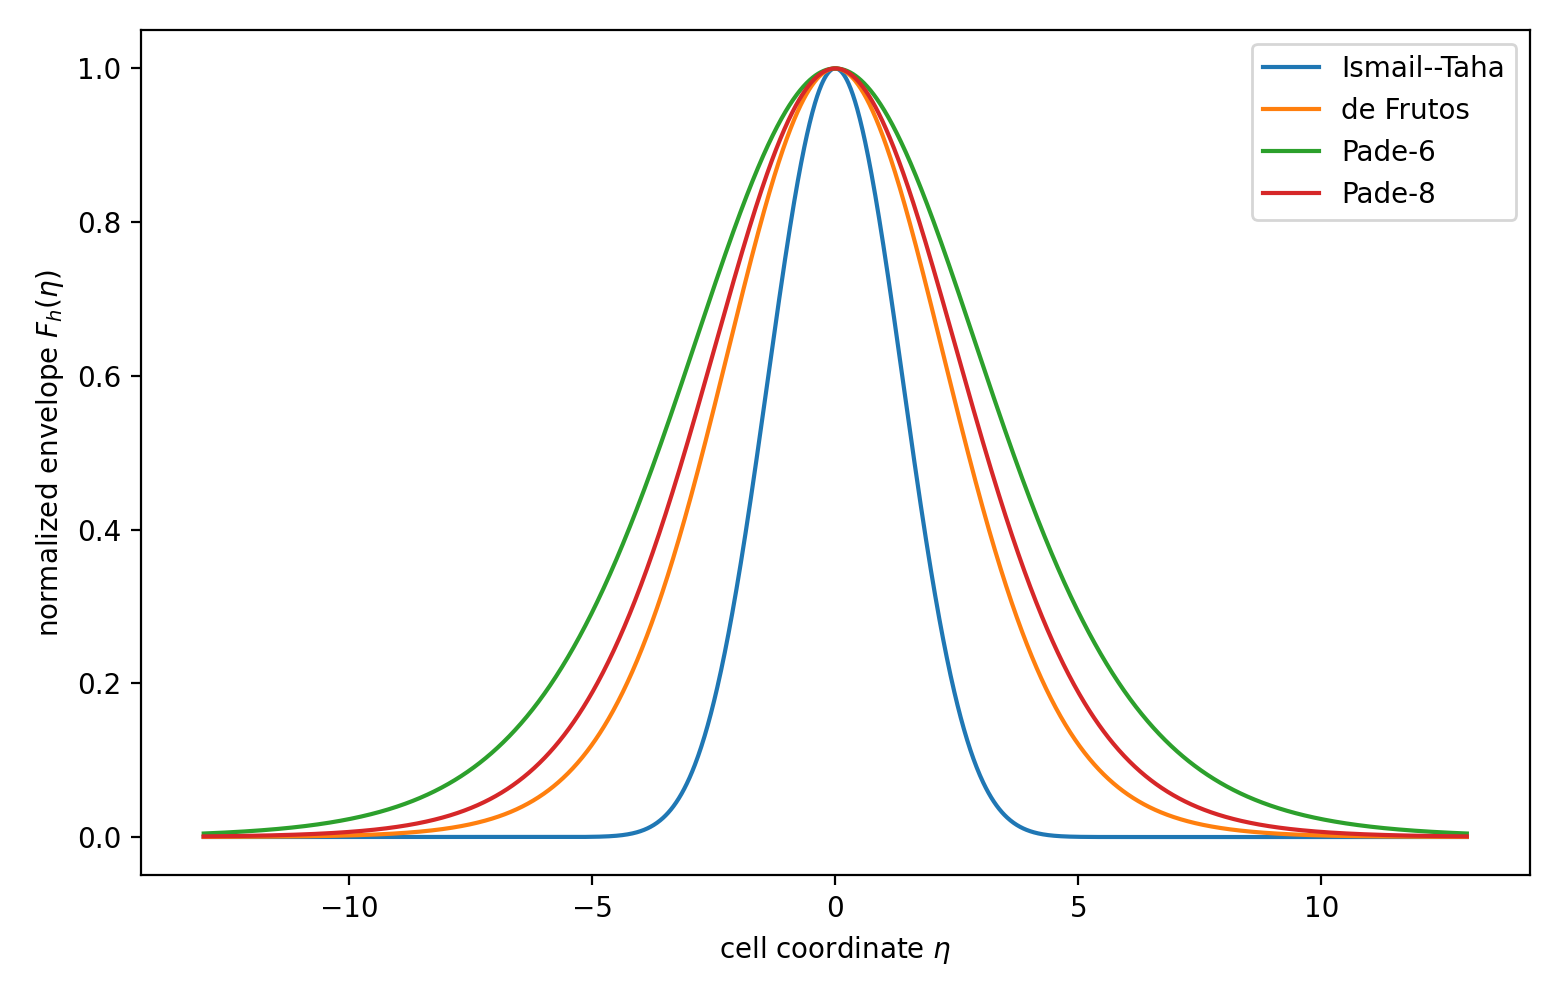
\includegraphics[width=0.76\textwidth]{wp4_nyquist_profiles.png}
 \caption{Normalized Nyquist solitary envelopes for the four spatial
 discretizations at $h=0.02$.  No width parameter is fitted.}
 \label{fig:wp4-profiles}
\end{figure}

The leading compacton-edge residual has the same antisymmetric phase factor
for all four methods but a different coefficient:
\begin{equation}
 D_N^{\rm IT}=\frac{2\phi-1}{24},\qquad
 D_N^{\rm DF}=\frac{2\phi-1}{180},\qquad
 D_N^{\rm P6}=\frac{2\phi-1}{360},\qquad
 D_N^{\rm P8}=\frac{2\phi-1}{280}.
 \label{eq:wp4-edge-seeds}
\end{equation}
Consequently the $O(h^2)$ seed scale is common, whereas the leading injection
coefficient is stencil dependent.

\subsection{Floquet instability for four independent stencils}

To avoid attributing the comparison to implicit midpoint, the principal
cross-stencil spectrum was computed with the fourth-order two-stage
Gauss--Legendre method at fixed edge phase $\phi_R=1/4$, $h=0.02$, and
$\kappa=10$.  All four numerical traveling compactons are unstable:
\begin{equation}
\begin{array}{c|c|c}
 \text{method} & \lambda_1 & \rho_F\\ \hline
 \text{Ismail--Taha} & -1.058004\pm0.141969\,\mathrm i &1.067486\\
 \text{de Frutos} & -1.134199 &1.134199\\
 \text{Pad\'e-6} & -1.155974 &1.155974\\
 \text{Pad\'e-8} & -1.132463 &1.132463
\end{array}
 \label{eq:wp4-floquet-table}
\end{equation}
The leading eigenpair residuals lie between $2.0\times10^{-12}$ and
$5.7\times10^{-11}$.  Independent midpoint calculations give the same
qualitative conclusion.  Hence edge--Floquet instability is not a special
property of the de Frutos mass matrix or derivative stencil, although the
multiplier and its real or complex character remain method dependent.

\begin{figure}[t]
 \centering
 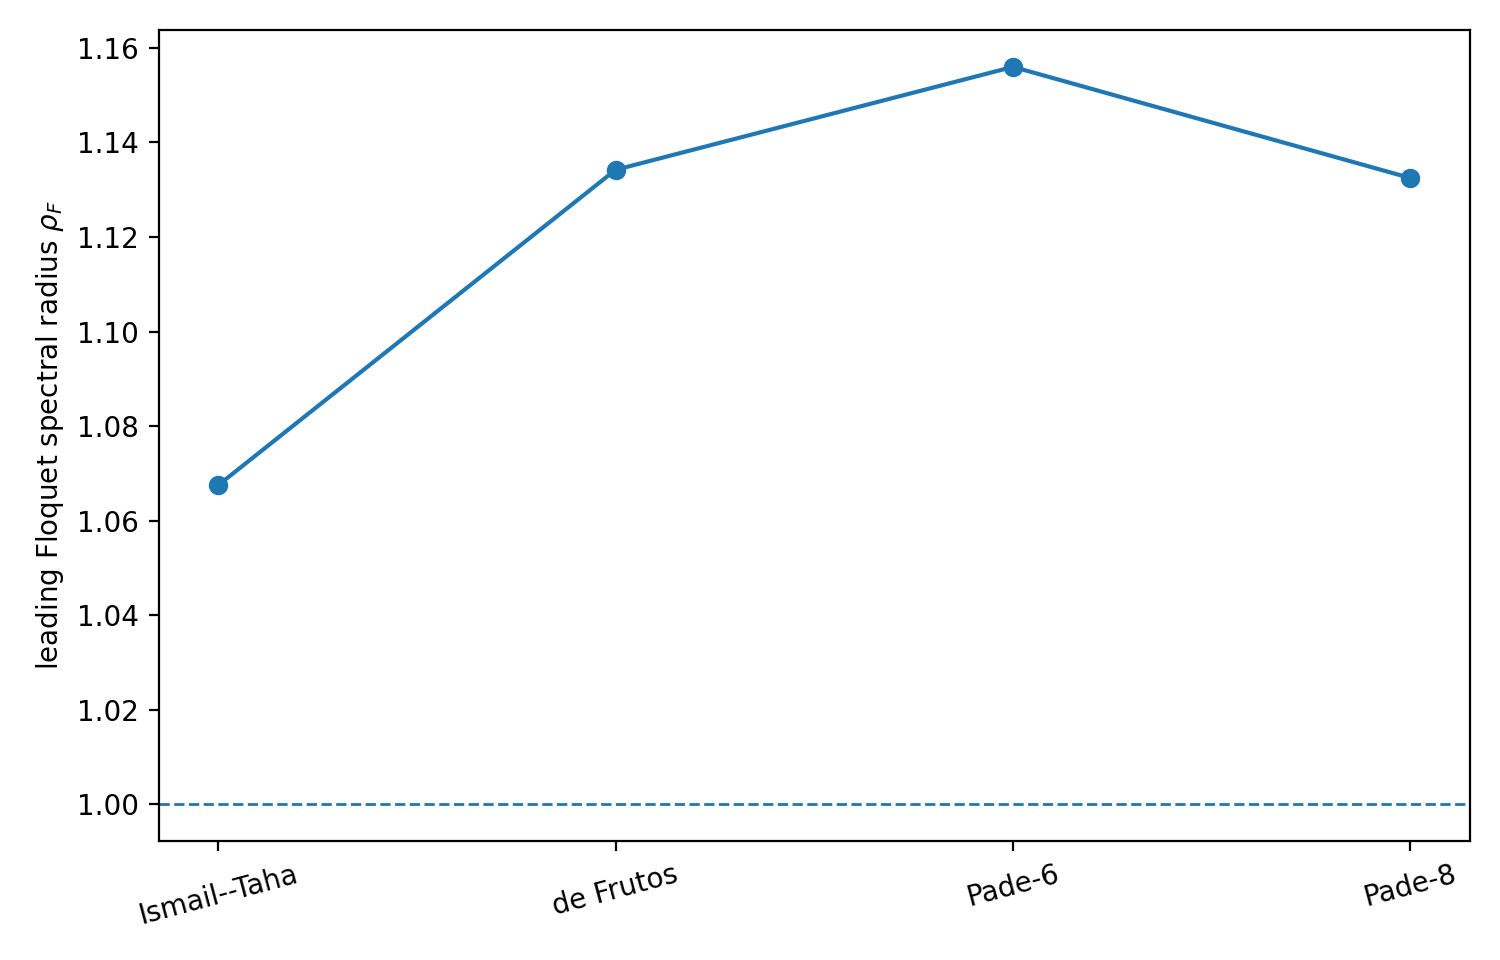
\includegraphics[width=0.68\textwidth]{wp4_spatial_floquet_GL4.png}
 \caption{Leading Floquet spectral radius for the four spatial methods,
 computed with GL4 at $h=0.02$, $\kappa=10$, and fixed edge phase.}
 \label{fig:wp4-floquet}
\end{figure}

\subsection{Natural shedding and stencil-specific capture}

Natural compacton runs were then performed with each stencil.  Ismail--Taha
produces a dense train of narrow forward packets, whereas Pad\'e-8 produces
wider and substantially faster packets.  Two clean tracks from each method
were fitted to the corresponding independently computed $F_{i,h}$.  The
median profile residuals are $1.14\times10^{-4}$ and $1.36\times10^{-4}$ for
the two Ismail packets, and $3.48\times10^{-4}$ and $2.66\times10^{-4}$ for
the Pad\'e-8 packets.  Their amplitudes and measured velocities are
\begin{equation}
\begin{array}{c|c|c}
 \text{packet} & A/h^2 & v_{\rm natural}\\ \hline
 \text{IT-I} &0.6525448&1.8634683\\
 \text{IT-II}&0.7125396&2.0345280\\
 \text{P8-I} &0.1471262&4.7011003\\
 \text{P8-II}&0.1286201&4.1109062
\end{array}
 \label{eq:wp4-natural-packets}
\end{equation}

As an independent test, free waves were initialized directly with the same
method-specific profiles and amplitudes.  Their velocities differ from those
of the naturally emitted packets by only $2.6\times10^{-5}$,
$3.1\times10^{-5}$, $8.8\times10^{-5}$, and $6.7\times10^{-5}$ in relative
terms.  Moreover, fitting a clean Ismail packet with any of the three wrong
profiles raises the residual from $1.16\times10^{-4}$ to at least $0.375$;
for a Pad\'e-8 packet the own-profile residual is $3.48\times10^{-4}$ and the
best wrong-profile residual is $0.0890$.  The captured object is therefore
not an arbitrary bell-shaped Nyquist pulse: it selects the nonlinear solitary
family of the actual stencil.

\begin{figure}[t]
 \centering
 \begin{minipage}{0.49\textwidth}
  \centering
  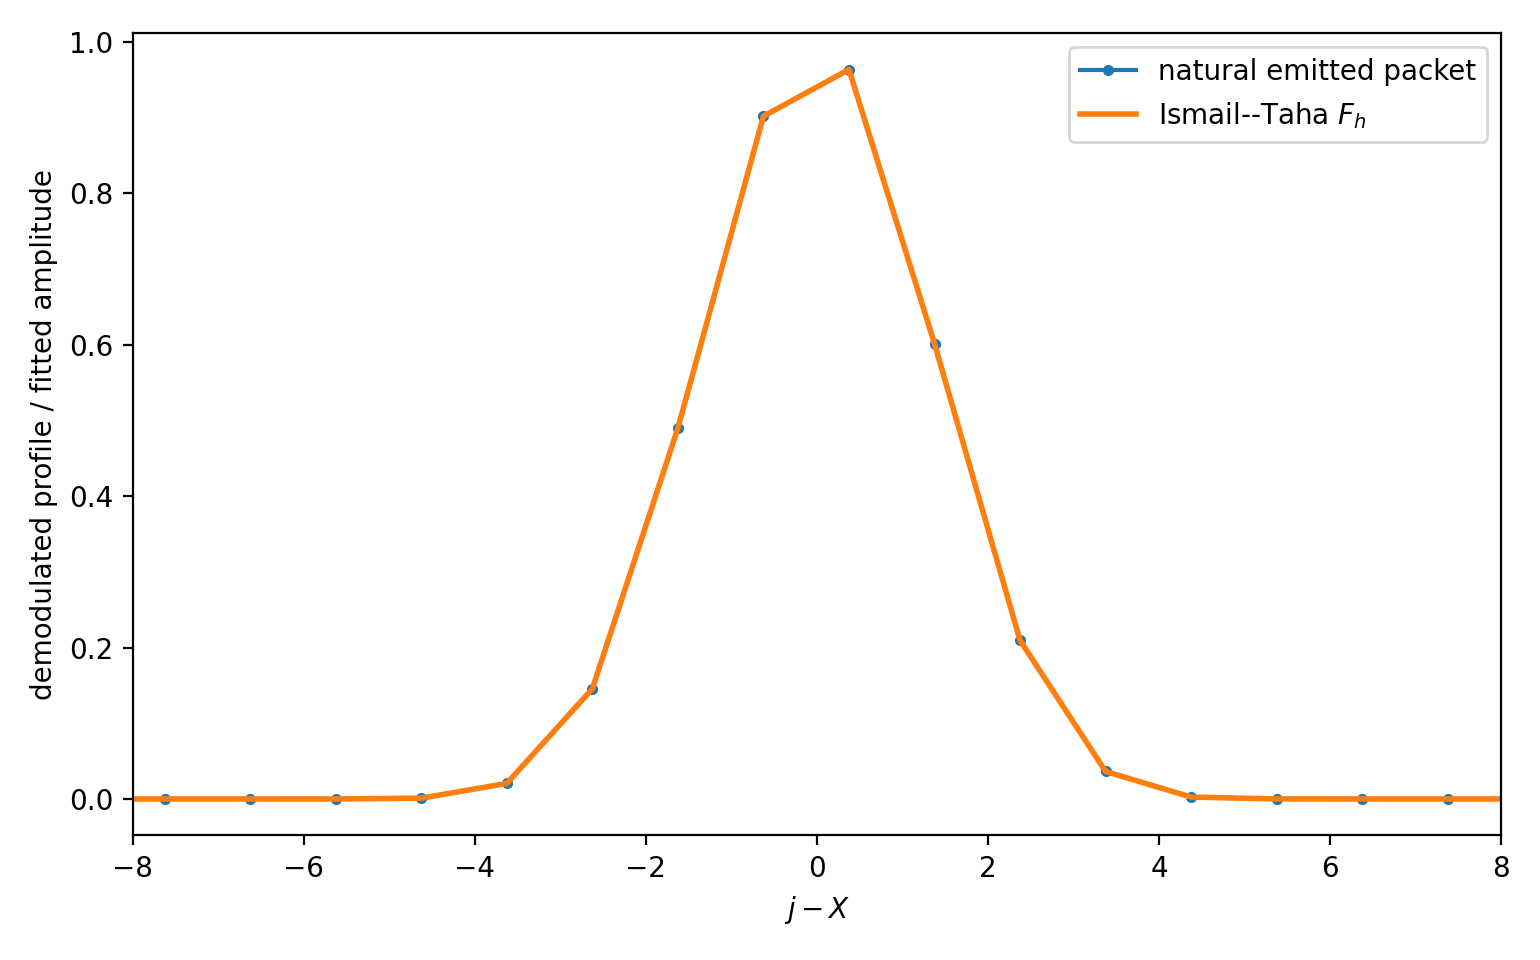
\includegraphics[width=\linewidth]{wp4_profile_capture_ismail.png}
 \end{minipage}\hfill
 \begin{minipage}{0.49\textwidth}
  \centering
  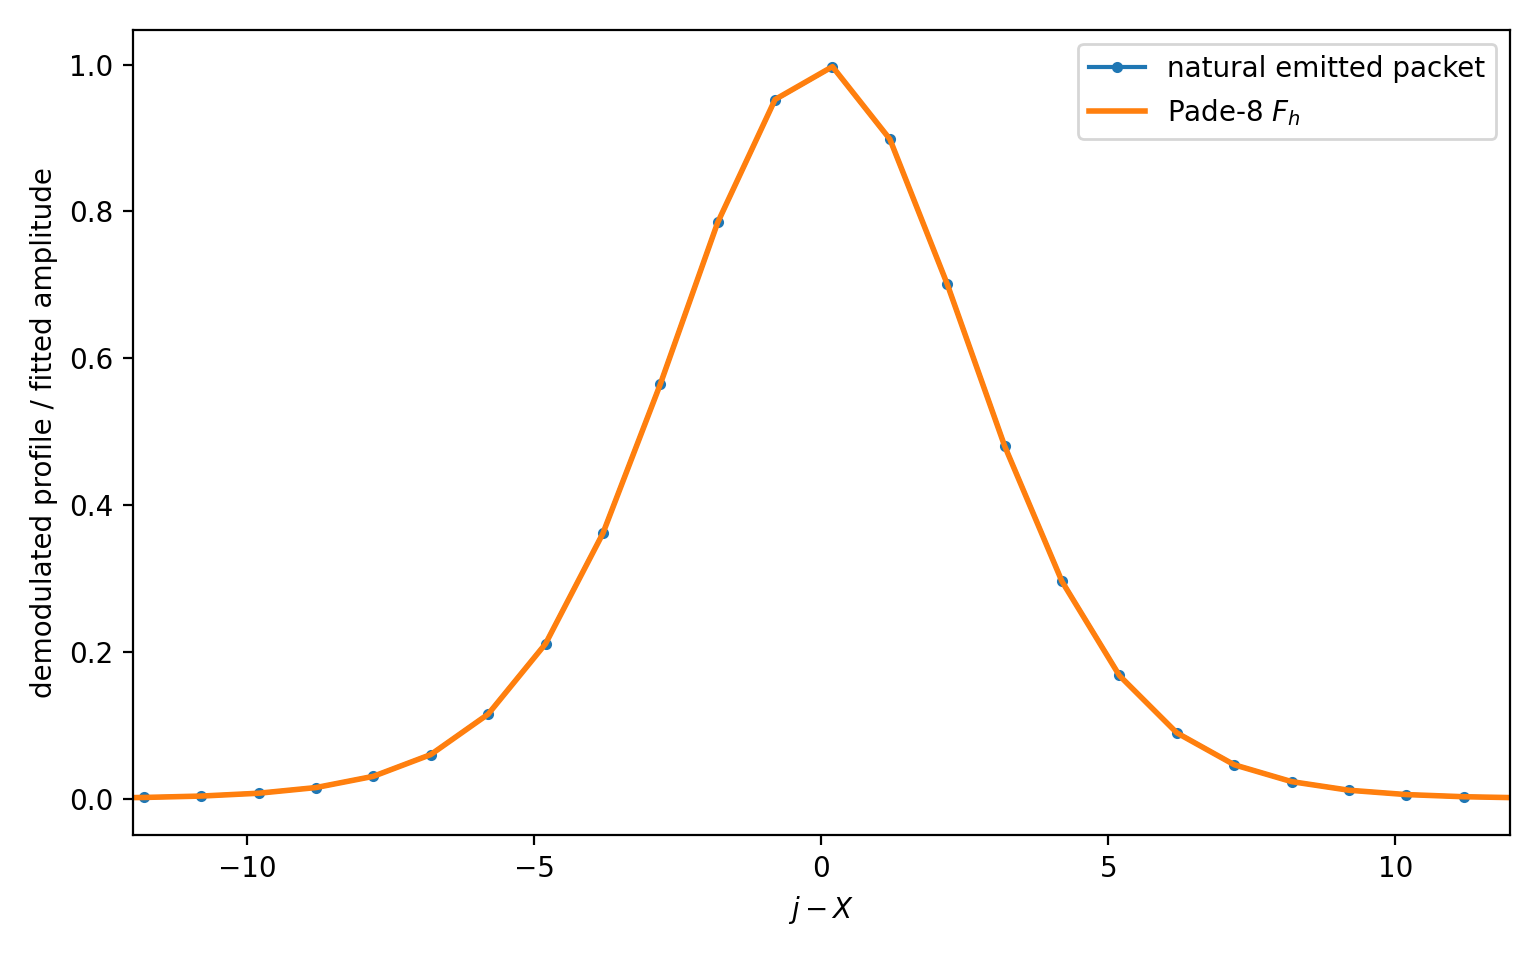
\includegraphics[width=\linewidth]{wp4_profile_capture_pade8.png}
 \end{minipage}
 \caption{Natural emitted packets captured by the method-specific Nyquist
 family.  Left: Ismail--Taha.  Right: Pad\'e-8.}
 \label{fig:wp4-capture}
\end{figure}

At the selected Pad\'e-6 phase the compacton is Floquet unstable but no clean
isolated packet with profile residual below $2\%$ appears by $T=30$.  This
finite-window negative result shows that $\rho_F>1$ is the linear trigger, not
a complete scalar prediction of shedding latency or packet isolation.

The comparison therefore separates the robust mechanism from its numerical
realization.  Exact Nyquist reduction, the $O(h^2)$ edge seed, edge--Floquet
instability, and nonlinear discrete-wave capture persist across independent
compact stencils.  The envelope kernel, velocity coefficient, seed strength,
Floquet branch, and nonlinear shedding chronology are all method dependent.
